HTBAC is a software system for running ensemble-based free energy protocols
adaptively and at scale on HPC resources. Currently, HTBAC supports protocols
composed of an arbitrary number of analysis and simulation steps, and relies
on the ensemble management system and runtime system provided by the
RADICAL-Cybertools (RCT). HTBAC is designed to be extended to support more
types of protocols and alternative runtime middleware.

% A -------------------------------------------------------------------------
\subsection{Requirements}

HTBAC satisfies three main requirements: (1) enable the scalable execution of
concurrent free energy protocols; (2) abstract protocol specification from
execution and resource management; and, (3) enable adaptive execution of
protocols.

Computational drug campaigns increasingly depend on scalable ensemble-based
protocols. This poses at least two major computational challenges. First,
ensemble-based protocols require execution coordination and resource
management among ensemble members, within protocols as well as across
protocols. Second, the setup of execution environments and data management
has to preserve efficient resource utilization. These challenges need to be
addressed by HTBAC as well as the underlying ensemble management and runtime
system.

Adaptive execution of protocols require the ability to change the control
logic of the ensemble execution, based on intermediate results of the ongoing
computation. Thus, HTBAC has to support resource redistribution, according to
the logic of the adaptive algorithms, enabling the optimization of
computational efficiency.

Finally, usability plays an important role in the development of HTBAC. HTBAC
has to provide a flexible interface which enables users to easily scale the
number of drug candidates and quickly prototype existing and novel free
energy protocols.

% B -------------------------------------------------------------------------
\subsection{Design and Implementation}\label{ssec:design_arch}

HTBAC exposes four constructs to specify free energy protocols: Protocol,
Simulation, Analysis, and Resource. \textbf{Protocol} enables multiple
descriptions of protocol types, while \textbf{Simulation} and
\textbf{Analysis} specify simulation and analysis parameters for each
protocol. \textbf{Resource} allows to specify the amount of resources needed
to execute the given protocols. Together, protocol instances, simulation and
analysis parameters, and resource requirements constitute an HTBAC
\textbf{application}.

Each protocol models a unique protein ligand physical system. Protocols
follow a sequence of simulation and analysis steps, assigning ensemble
members to execute independent simulations or analysis. An ensemble member
that executes a simulation within a simulation step is referred to as a
replica. Each simulation is assigned a different initial velocity, which
enables simulations to begin in different parts of the ligand's phase space.

Individual simulations or analyses with input, output, termination criteria
and dedicated resources are designed as a computational
\textbf{task}~\cite{power-of-many17}. Aggregates of tasks with dependencies
that determine the order of their execution constitute a \textbf{workflow}.
In this way, HTBAC encodes $N_P$ instances of the P$^{th}$ protocol as a
workflow of computational tasks.

Fig.~\ref{fig:architecture} shows the components and subcomponents of HTBAC.
The API enables users to describe protocols in terms of protocol type,
simulation and analysis steps, and compute infrastructure requirements. The
Descriptor component uses two subcomponents to aggregate protocol
descriptions into a single application and resource description. Note that
Descriptor can aggregate different types of protocols, with different
computing and resource requirements.

\begin{figure}
  \centering
  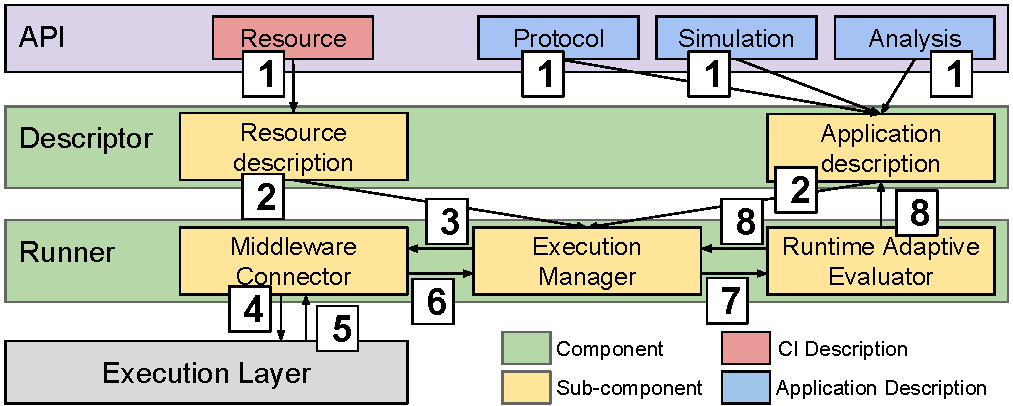
\includegraphics[width=\columnwidth]{figures/HTBAC_architecture_model.pdf}
  \caption{HTBAC architecture. Users specify protocol(s) with multiple
  simulation and analysis steps. Descriptor derives a single application that
  Runner executes on an external execution layer. Runtime Adaptive Evaluator
  enables the execution of adaptive protocols.}\label{fig:architecture}
\up{}
\up{}
\end{figure}

The Runner component has three subcomponents: Execution Manager, Middleware
Connector and Runtime Adaptive Evaluator. Execution Manager communicates with
the execution layer via a connector to coordinate the execution of the
application. In principle, HTBAC can use multiple connectors for diverse
middleware to access different computing infrastructures.

Middleware Connector converts the application description of HTBAC into a
middleware-specific format. Execution Manager can pass the given application
to the connector in full or only in parts. This enables to start the
execution of an application before its full description is available or to
change those parts of the application that still have to be executed. This
will enable future capabilities like, for example, to concurrently execute
the application on diverse middleware.

Runtime Adaptive Evaluator enables the execution of adaptive applications.
This subcomponent can evaluate partial results of an application execution
via tailored algorithms. On the base of this evaluation, Runtime Adaptive
Evaluator can decide to return the control to Execution Manager or to modify
the description of the application that is being executed. In this way, HTBAC
implements adaptivity for diverse protocols, allowing users to define
arbitrary conditions and algorithms.

HTBAC is implemented in Python as a domain-specific library. All components
of HTBAC are implemented as objects that communicate via method calls. HTBAC
uses two RCT as building blocks~\cite{review_bb_2016}: Ensemble Toolkit
(EnTK) and RADICAL-Pilot (RP).

EnTK provides HTBAC capabilities to execute ensemble-based
applications~\cite{power-of-many17}. EnTK exposes three constructs:
\textbf{Task}, \textbf{Stage} and \textbf{Pipeline}. Tasks contain
information regarding an executable, its software environment and its data
dependencies. Stages are sets of tasks without mutual dependencies that can
execute concurrently. Pipeline are lists of stages, where stages can execute
only sequentially. Pipelines can execute independently. HTBAC uses a
Middleware Connector for EnTK to encode a protocol instance as a single
pipeline that contains stages of individual simulations and analyses tasks.

EnTK is designed to be coupled with different runtime systems. In this paper,
EnTK uses RP to execute tasks via pilots. RP supports task-level parallelism
and high-throughput by acquiring resources from a computing infrastructure
and scheduling tasks on those resources for execution. RP uses RADICAL SAGA
to interface with several resource managers, including SLURM, PBS (pro), and
LSF. Pilot systems execute tasks directly on the resources, without queuing
them on the infrastructure's scheduler.

% C -------------------------------------------------------------------------
\subsection{Execution Model}\label{ssec:adaptive_execution}

Users describe one or more protocols alongside their
resource requirements via HTBAC's API. Descriptor takes these descriptions as
input and returns an application description (Fig.~\ref{fig:architecture}.1).
As seen in \S\ref{ssec:design_arch}, this application consists of a set or
sequence of tasks with a set of resource requirements for their execution.

The application description is passed to the Execution Manager of the Runner
component (Fig.~\ref{fig:architecture}.2). Execution Manager evaluates the
resource requirements, selects a suitable connector (currently only to EnTK),
tags each protocol instance of the application with an ID, and passes all or
part of the application description to the connector for execution
(Fig.~\ref{fig:architecture}.3).

The Middleware Connector of the Runner component gets the application
description, converting it into a middleware-specific description (EnTK
pipelines of stages of tasks) and a resource request. The connector submits
this request to the underlying execution layer
(Fig.~\ref{fig:architecture}.4) and initiates the execution of the
application once the execution layer communicates the availability of the
resources (Fig.~\ref{fig:architecture}.5).

The resource requirements specified via HTBAC's API include walltime, cores,
queue, and user credentials. EnTK derives a resource request from these
requirements, converting it into a pilot description for RP. RP converts this
pilot requests into a batch script that is submitted to the specified HPC
machine. Once the pilot becomes active, EnTK identifies those application
tasks that have satisfied dependencies and can be executed concurrently.
EnTK's own Execution Manager uses RP to execute those tasks on pilot's
resources.

HTBAC allows to specify conditions tailored to individual simulation steps of
a protocol implementation. We leverage this ability to implement adaptivity
by enabling the user to partition protocols into simulation steps and
generate new simulation steps at runtime, based on a set of predefined
conditions. The user specifies these conditions in an analysis script for the
Runtime Adaptive Evaluator subcomponent.

Execution Manager can retrieve the results of simulations
(Fig.~\ref{fig:architecture}.6) and these results can be evaluated by Runtime
Adaptive Evaluator via a user-defined analysis script
(Fig.~\ref{fig:architecture}.7). Depending on the result of the evaluation,
Runtime Adaptive Evaluator may generate new simulation steps, adding them to
the application description (Fig.~\ref{fig:architecture}.8a) or return the
control to Application Manager (Fig.~\ref{fig:architecture}.8b) without
changing the application. If new simulations are to be generated, the
Execution Manager bypasses termination of the application, and passes the
added application description to the connector.

% Execution Manager uses the protocols' ID to keep track of those protocols
% that require additional simulations at runtime. In this way, older
% simulations can continue executing while new simulations can be passed to
% the Execution Manager.

In an adaptive scenario, as the number of simulations grows at runtime, the
ratio of cores-to-task fluctuates. EnTK's Execution Manager automatically
redistributes an even share of the total requested cores to each simulation.
RP allows for new simulations to execute within the pilot's wall-time,
without having to acquire new resources via the resource management system.

% D -------------------------------------------------------------------------
\subsection{Implementing ESMACS and TIES in
HTBAC}\label{sec:implementation_htbac}

In \S\ref{ssec:esm_ties} we define the structure of the ESMACS and TIES
protocols. Here we provide skeletons of the TIES protocol implemented in
HTBAC\@. In L.~\ref{lst:ties.py} we show a customization of a production
MD simulation step.

\lstinputlisting[language=Python, label={lst:ties.py}, caption={TIES protocol
implemented with HTBAC. We import the predefined protocol `TIES'. We assign
the physical system to the protocol, we instantiate a simulation, customize
its steps (\texttt{replica}, \texttt{lambda}) and assign it to the TIES's
\texttt{step0}. We instantiate Runner with a resource request and pass the
protocol to it.}]{ties.py}

In \S\ref{ssec:adaptive_execution} we show HTBAC's adaptive execution
capabilities. In L.~\ref{lst:ties_adaptivity.py} we provide an
intra-protocol adaptive implementation of TIES, based on the use-case
of \S\ref{ssec:adapt_ties}.

\lstinputlisting[language=Python, label={lst:ties_adaptivity.py},
caption={Adaptive TIES protocol implemented with HTBAC. Assuming
L.~\ref{lst:ties.py}, we run Runner retrieving runtime results, we specify an
adaptivity script for the evaluator, create TIES's \texttt{step1}. The
analysis script operates on partial simulation results, generating new
simulation conditions for the next simulation step.}]{ties_adaptivity.py}